\documentclass[11pt]{article}
\usepackage[utf8]{inputenc}

\usepackage{geometry}
\geometry{a4paper}

\usepackage{graphicx}
\usepackage{hyperref}
\usepackage[parfill]{parskip}
\usepackage{amsmath, amssymb}
\usepackage{fdsymbol}
\usepackage{color,soul}

% remove section numbering
\makeatletter
\renewcommand{\@seccntformat}[1]{}
\makeatother

% make subsubsection italic
\usepackage{sectsty}
\subsubsectionfont{\itshape}

\renewcommand{\arraystretch}{1.4}

\title{Probability Theory \& Statistics}
\date{}
\author{}

\begin{document}
\maketitle
\clearpage

\section{Beta-Binomial Conjugacy}

\subsection{Prerequisites}

\begin{itemize}
\item
Random Variables and their Distributions
\end{itemize}

\subsubsection{Recap}

\emph{Random variables} are \emph{functions} 
mapping the sample space, \(S\), 
to the real number line, \(\mathbb{R}\). 
For example, 
consider a coin-tossing problem. 
The structure of the problem is a sequence of trials 
with two possible outcomes for each trial. 
The outcomes are either heads (\(H\)) or tails (\(T\)), 
or equivalently ``success'' or ``failure'', 
or ``1'' or ``0''.

\begin{figure}[h!]
\centering
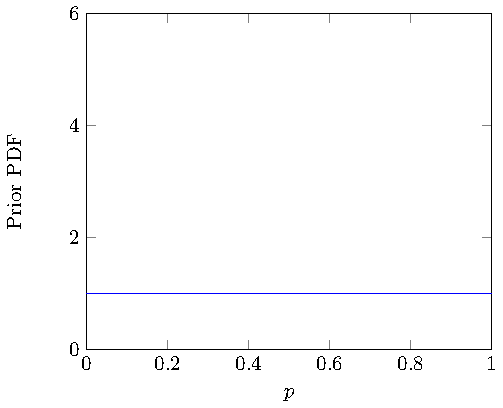
\includegraphics[width=0.75\linewidth]{tikz/figure1}
\caption{The function \(X\), mapping \(s_{j}\) to the real number line.}
\label{fig:mapping}
\end{figure}

For an experiment where the coin is flipped twice, 
the sample space consists of four possible outcomes
\begin{align}
S = \{HH, HT,TH, TT\}
\end{align}
that can also be mapped to a set of numbers. 
Figure \ref{fig:mapping} is one possible mapping, \(X(s_{j})\), 
from the sample space to the real number line, i.e.,
\begin{align}
X(HH) = 2,\ X(HT) = X(TH) = 1,\ X(TT) = 0
\end{align}
where the mapping corresponds 
to the total number of heads in the experiment. 
Notice how the mapping is somewhat arbitrary. 
We could have also defined a mapping on 
the same sample space counting the number of tails.

\subsubsection{Distributions}

The \emph{distribution} of a random variable \(X\), 
is a full description of the probabilities of the events associated with \(X\),
e.g., \(\{ X = 2\}\) and \(\{ 0 \leq X \leq 2\}\). 
The distribution of a \emph{discrete} random variable can be defined either 
by its \emph{Probability Mass Function} (PMF) or 
its \emph{Cumulative Distribution Function} (CDF). 
The PMF of a discrete random variable, \(X\), is the function
\begin{align}
P(A) = P\left( \left\{ X = x \right\} \right) = P(X = x)
\end{align}
for \(x \in \mathbb{R}\). 

For example, 
consider a 2-flip coin experiment,
\begin{align}
P(X = 2) = 
P\left( \{ X(s) = 2\} \right) = 
P\left( \left\{ X(s_{1}) \right\} \right) = 
P(\left\{ s_{1} \right\}) = 1/4
\end{align}
The CDF of \(X\) is the function
\begin{align}
P(B) = 
P\left( \left\{ X \leq x \right\} \right) = 
P(X \leq x).
\end{align}
For a 2-flip coin experiment we get,
\begin{align}
P(X \leq 2) = 
P\left( \left\{ X(s) \leq 2 \right\} \right) = 
P\left( \left\{ X\left( s_{1} \right), X\left( s_{2} \right), X\left( s_{3} \right), X\left( s_{4} \right) \right\} \right) = 
P\left( \left\{ S \right\} \right) = 1.
\end{align}
A PMF is \emph{valid} if it is nonnegative and sums to 1. 
A CDF is valid if it is right-continuous and increasing, 
and if it converges to 0 as \(x\) tends to \(- \infty\), 
and converges to 1 as \(x\) tends to \(\infty\).

A random variable has a \emph{continuous distribution} if its 
CDF is \emph{differentiable}.%
\footnote{Excluding endpoints.} 
A \emph{continuous random variable} is a random variable with a continuous distribution. 
It is often much more convenient to work 
with the derivative of a continuous CDF, 
a function called the \emph{Probability Density Function} (PDF)
\begin{align}
f(x) = F^\prime(x) = \frac{d}{dx}P(X \leq x)
\end{align}
where \(F(x)\) is the CDF of a continuous random variable \(X\).

% up to here

\subsubsection{Bernoulli and Binomial Discrete Distributions}

A random variable \(X\) has a \emph{Bernoulli distribution} 
with parameter \(p\) if \(P(X = 1) = p\), 
and \(P(X = 0) = 1 - p\), 
where \(0 < p < 1\).

We write this as
\begin{align}
X \sim Bern(p)
\end{align}
where the symbol \(\sim\) is read as ``is distributed as''. 
An experiment that can result in either 
a ``success'' or a ``failure'' but not \emph{both} 
is a called a \emph{Bernoulli trial}. 
A Bernoulli random variable is the indicator of a success or failure.

Suppose that \(n\) independent Bernoulli trials are performed, 
each with the same success probability \(p\). 
Let \(X\) be the number of successes. 
The distribution of \(X\) is called the \emph{Binomial distribution} 
with parameters \(n\) and \(p\). 
We write
\begin{align}
X \sim Bin(n,p)
\end{align}
when a random variable \(X\) has a \emph{Binomial distribution}. 
If \(X \sim Bin(n,p)\), 
the PMF of \(X\) is
\begin{align}
P(X = k) = \binom{n}{k}p^{k}(1 - p)^{k} = 
\binom{n}{k}p^{k}(1 - p)^{n - k}.
\end{align}

\subsubsection{Beta Continuous Distribution}

A random variable \(X\) has a \emph{Beta distribution} with parameters \(a\) and \(b\), 
where \(a > 0\) and \(b > 0\), 
if its PDF is
\begin{align}
f(x) = \frac{1}{\beta(a,b)}x^{a - 1}(1 - x)^{b - 1},\ \ 0 < x < 1,
\end{align}
where the constant \(\beta(a,b)\) is chosen to make the PDF integrate to 1. 
We write this as
\begin{align}
X \sim Beta(a,b).
\end{align}

\subsection{Bayesian Inference}

Suppose we have a coin that lands heads with probability \(p\), 
but we do not know the value of \(p\). 
Our goal is to \emph{infer} the value of \(p\) after observing \(n\) coin tosses. 
Ideally, 
the more observations we make, 
the better our estimate.

\emph{Bayesian inference} treats all unknown quantities as random variables. 
Therefore, 
in the above described problem, 
we treat \(p\) as a \emph{random variable} and give it a \emph{distribution}. 
The distribution we give to \(p\) reflects our uncertainty about the 
true value of \(p\) before we observe any coin tosses. 
We call this distribution, 
the \emph{prior distribution}. 
After observing an experiment, 
and the data from the experiment have been collected, 
the prior distribution is updated using Bayes' rule. 
This yields the \emph{posterior} distribution that now reflects 
our new beliefs about \(p\).

\subsubsection{Beta-Gamma Conjugacy}

Suppose our \emph{prior belief} about the true value of \(p\), 
the probability a coin lands heads, 
is described by the \emph{beta distribution}
\begin{align}
p \sim Beta(a,b)
\end{align}
where \(a\) and \(b\) are \emph{known constants}.

Next, 
let \(X\) be the number of heads in \(n\) coin tosses. 
Knowing the true value of \(p\) means that each realization of \(X\) is an 
independent Bernoulli trial with a \(p\) probability of success
\begin{align}
X|p \sim Bin(n,p)
\end{align}
Note, 
\(X\) is not \emph{marginally} Binomial, 
it is \emph{conditionally} Binomial. 
Its marginal distribution is called the \emph{Beta-Binomial distribution.}

We can update our belief, 
after observing data, 
using Bayes' rule (in hybrid form) 
in exactly the same way we did in the \emph{biased coin problem}. 
Letting \(f(p)\) be the prior distribution,%
\footnote{Note how we have 
switched ``probability'' for ``distribution'' compared 
to the previous session's definition. 
It is not trivial to prove, 
but it can be shown that a general rule applies.} 
and \(f(p|X = k)\) be the \emph{posterior distribution} after observing \(k\) heads
\begin{align}
f\left( p \middle| X = k \right) = 
\frac{P\left( X = k \middle| p \right) \cdot f(p)}{P(X = k)}
\end{align}
Using the definitions of the Beta and Binomial distributions from the previous sections,
\begin{align}
f\left( p \middle| X = k \right) = 
\frac{\binom{n}{k}p^{k}(1 - p)^{n - k} \cdot \frac{1}{\beta(a,b)}x^{a - 1}(1 - x)^{b - 1}}{P(X = k)}
\end{align}
The denominator, 
the \emph{marginal distribution} of \(X\), 
is obtained by integrating over the support of the 
\emph{conditional distribution} (equivalently the joint distribution 
by the definition of conditional probability)
\begin{align}
P(X = k) = \int_{0}^{1}{P\left( X = k \middle| p \right)f(p)dp} = 
\int_{0}^{1}{\binom{n}{k}p^{k}(1 - p)^{n - k}f(p)dp}.
\end{align}
For \(a = b = 1\), and
\begin{align}
p \sim Unif(0,1)
\end{align}
so that \(f(p) = \frac{x}{b - a}\), 
it can be shown that \(P(X = k)\) has a \emph{Discrete Uniform distribution}. 
For general \(a\) and \(b\) the problem seems difficult.

The posterior distribution \(f(p|X = k)\) is a function of \(p\), i.e.,
\begin{align}
f\left( p | X = k \right) = g(p)
\end{align}
which means that everything that does not depend on \(p\) is a constant.
We can therefore drop all of the constant terms in the expression and
determine the normalizing constant to be whatever is needed to make the
PDF integrate to 1. 
This gives
\begin{align}
f\left( p | X = k \right) \propto 
p^{a + k + 1} \cdot (1 - p)^{b + n - k - 1},
\end{align}
which is the \(Beta(a + k,b + n - k)\) PDF, 
up to a multiplicative constant! 

This special relationship between the Beta and Binomial distributions is known as \emph{conjugacy}. 
Beta is the conjugate prior of the Binomial, 
which means that if we have a Beta prior distribution on \(p\) 
and the data are conditionally Binomial given \(p\), 
when going from prior to posterior, 
we do not leave the family of Beta distributions.

\subsubsection{Example}

Suppose our prior belief about the true value of \(p\), 
the probability a coin lands heads, 
is described by the prior \(Beta(1,1)\), 
which is equivalent to a \(Unif(0,1)\) distribution. 
This assigns an equal probability to any value of \(0<p<1.\) 
In words, 
we don't assume anything about \(p\) since any \(p \in [0,1]\) is 
equally likely.%
\footnote{Technically, 
the probability \(p\) falls in an equal length disjoint partition of the interval where 
the probability is proportional to the length of the subset.}
Note, 
this doesn't mean the prior is \emph{uninformative}, 
knowing the probability is equally likely means we still know something.

After \(n = 5\) coin tosses we observe \(k = 5\) Heads. 
The posterior then is \(Beta(6,1)\) plotted in Figure \ref{fig:prior}

\begin{figure}[h!]
\centering
\begin{minipage}{.5\textwidth}
  \centering
  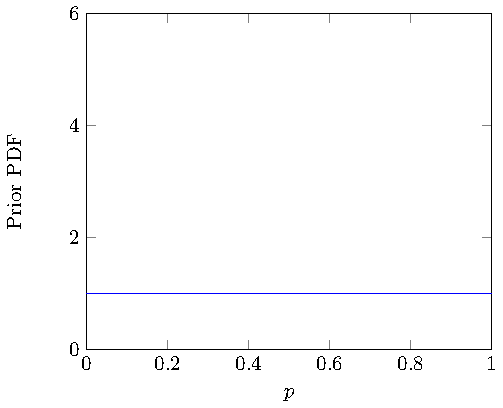
\includegraphics[width=0.9\linewidth]{tikz/figure1}
\end{minipage}%
\begin{minipage}{.5\textwidth}
  \centering
  
\includegraphics[width=0.9\linewidth]{tikz/figure2}
\end{minipage}
\caption{%
Uniform prior (left) and posterior \(Beta(6,1)\) of bias in 
coin after 5 heads in 5 tosses are observed.}
\label{fig:prior}
\end{figure}

This model is the continuous analogue of the 
\emph{biased coin problem} from the conditional probability session. 
In the biased coin problem, 
we also had a coin with probability of heads \(p\) that was unknown, 
but our prior information led us to believe that \(p\) could only take on one of two values: 1/2 or 3/4. 
The prior distribution, 
although we did not call it that, 
was discrete
\begin{align}P\left( p = \frac{1}{2} \right) = 1/2\end{align}
\begin{align}P\left( p = \frac{3}{4} \right) = 1/2\end{align}
After observing 3 heads, 
we obtained the posterior PMF that assigned 0.23 to \(p = 1/2\) and 0.77 to \(p = 3/4\). 
The same logic applies here, 
only \(p\) can take on any value between 0 and 1.

\section{Practice}

\subsection{Biased Coins}

1) Draw the prior and posterior PMFs for the biased coin problem in its discrete form.

\subsection{Clinical Trials}

A new treatment has just been developed for a disease. 
A clinical trial is about to be conducted to study how effective the treatment is. 
The treatment will be applied to \(n\) patients who have the disease. 
Given \(p\), 
the patients' outcomes are independent, 
with each patient having probability \(p\) of being cured by the treatment. 
But \(p\) is unknown. 
To quantify our uncertainty about \(p\), 
we model \(p\) as a random variable, 
with prior distribution \(p \sim Unif(0,1)\).

1) Find the probability that exactly \(k\) out of the \(n\) patients will be 
cured by the treatment (unconditionally, \emph{not} given \(p\)).

2) Suppose the treatment is extremely effective in the clinical trial: all \(n\) patients are cured! 
Given this information, find the probability that \(p\) exceeds 1/2.

\end{document}
